%!TEX root = ../../common/main.tex

\chapter{Studies of systematic effects}
\label{ch:app:measurement_of_sin2beta:systematics}

% %%%%%%%%%%%%%%%%%%%%%%%%%%%%%%%%%%%%%%%%%%%%%%%%%%%%%%%%%%%%%%%%%%%%%%%%%%%%%%
\section{Systematics}
\label{sec:app:measurement_of_sin2beta:systematics:systematics}

% ------------------------------------------------------------------------------
\subsection{Fit model}
\label{sec:app:measurement_of_sin2beta:systematics:systematics:fit_model}

% ------------------------------------------------------------------------------
\subsection{Flavour Tagging}
\label{sec:app:measurement_of_sin2beta:systematics:systematics:tagging}

% ------------------------------------------------------------------------------
\subsection{Decay time resolution}
\label{sec:app:measurement_of_sin2beta:systematics:systematics:resolution}

% ------------------------------------------------------------------------------
\subsection{Decay time acceptance}
\label{sec:app:measurement_of_sin2beta:systematics:systematics:acceptance}

% ..............................................................................
\subsection{Low decay time acceptance}
\label{sec:app:measurement_of_sin2beta:systematics:systematics:acceptance:lower}

\begin{figure}[h]
  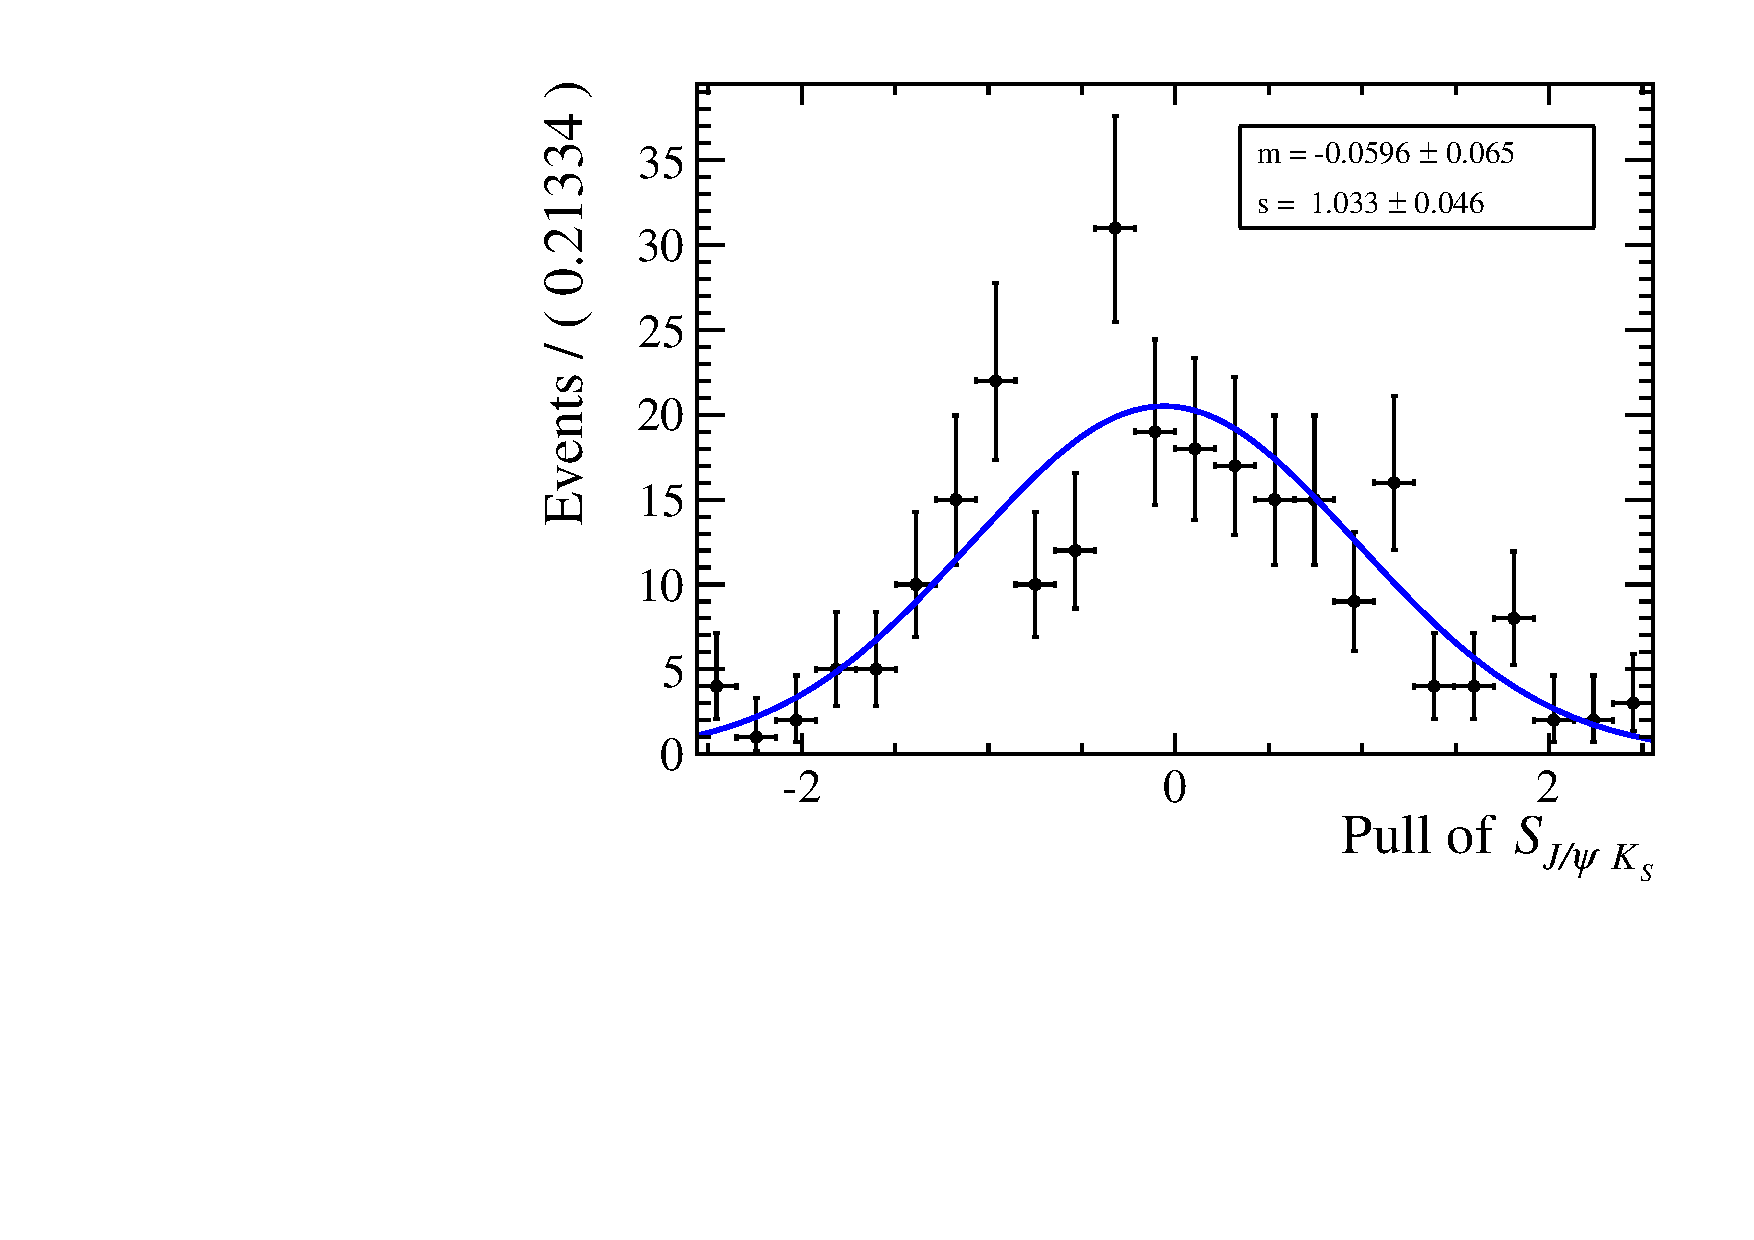
\includegraphics[width=0.49\textwidth]{private/content/measurement-of-sin2beta/figs/systematics_acc_lower_s_pull.pdf}\hfill
  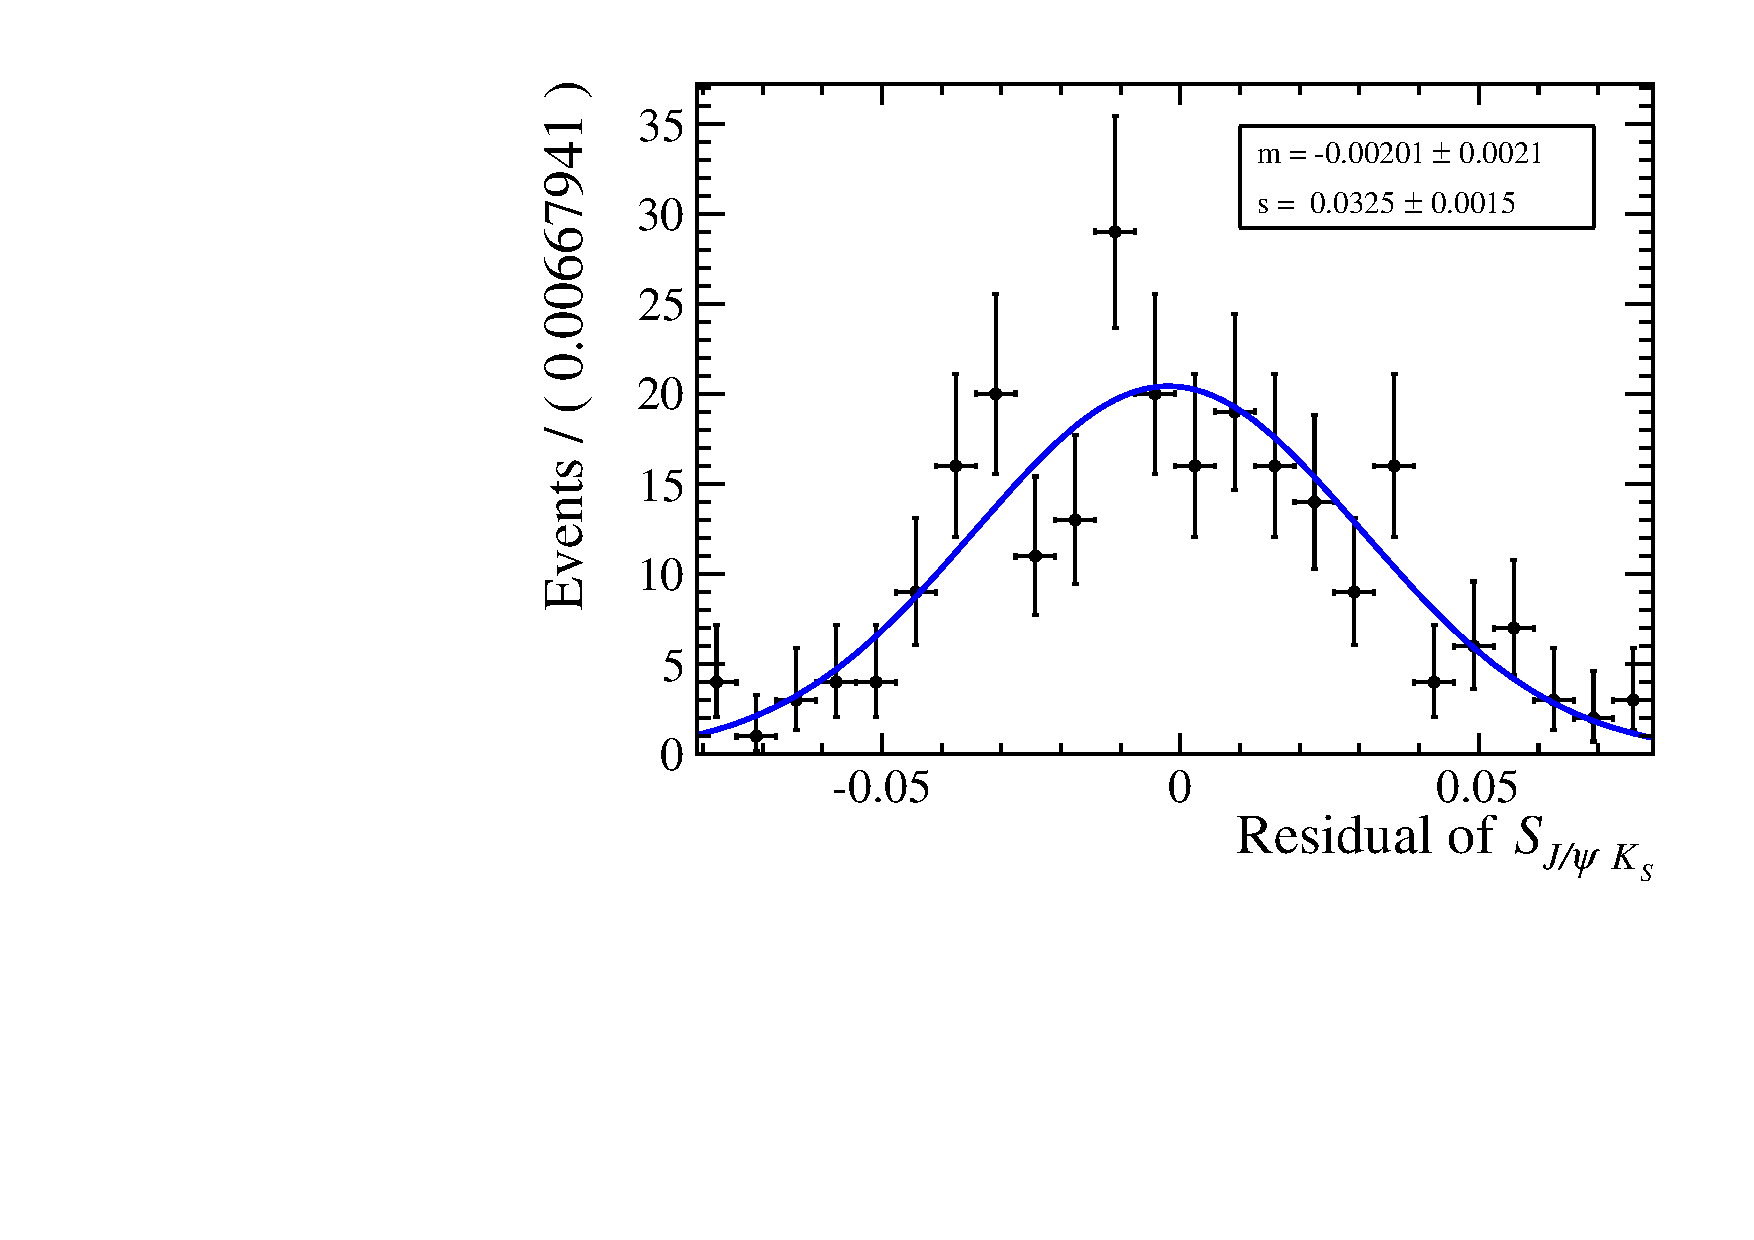
\includegraphics[width=0.49\textwidth]{private/content/measurement-of-sin2beta/figs/systematics_acc_lower_s_res.pdf}
  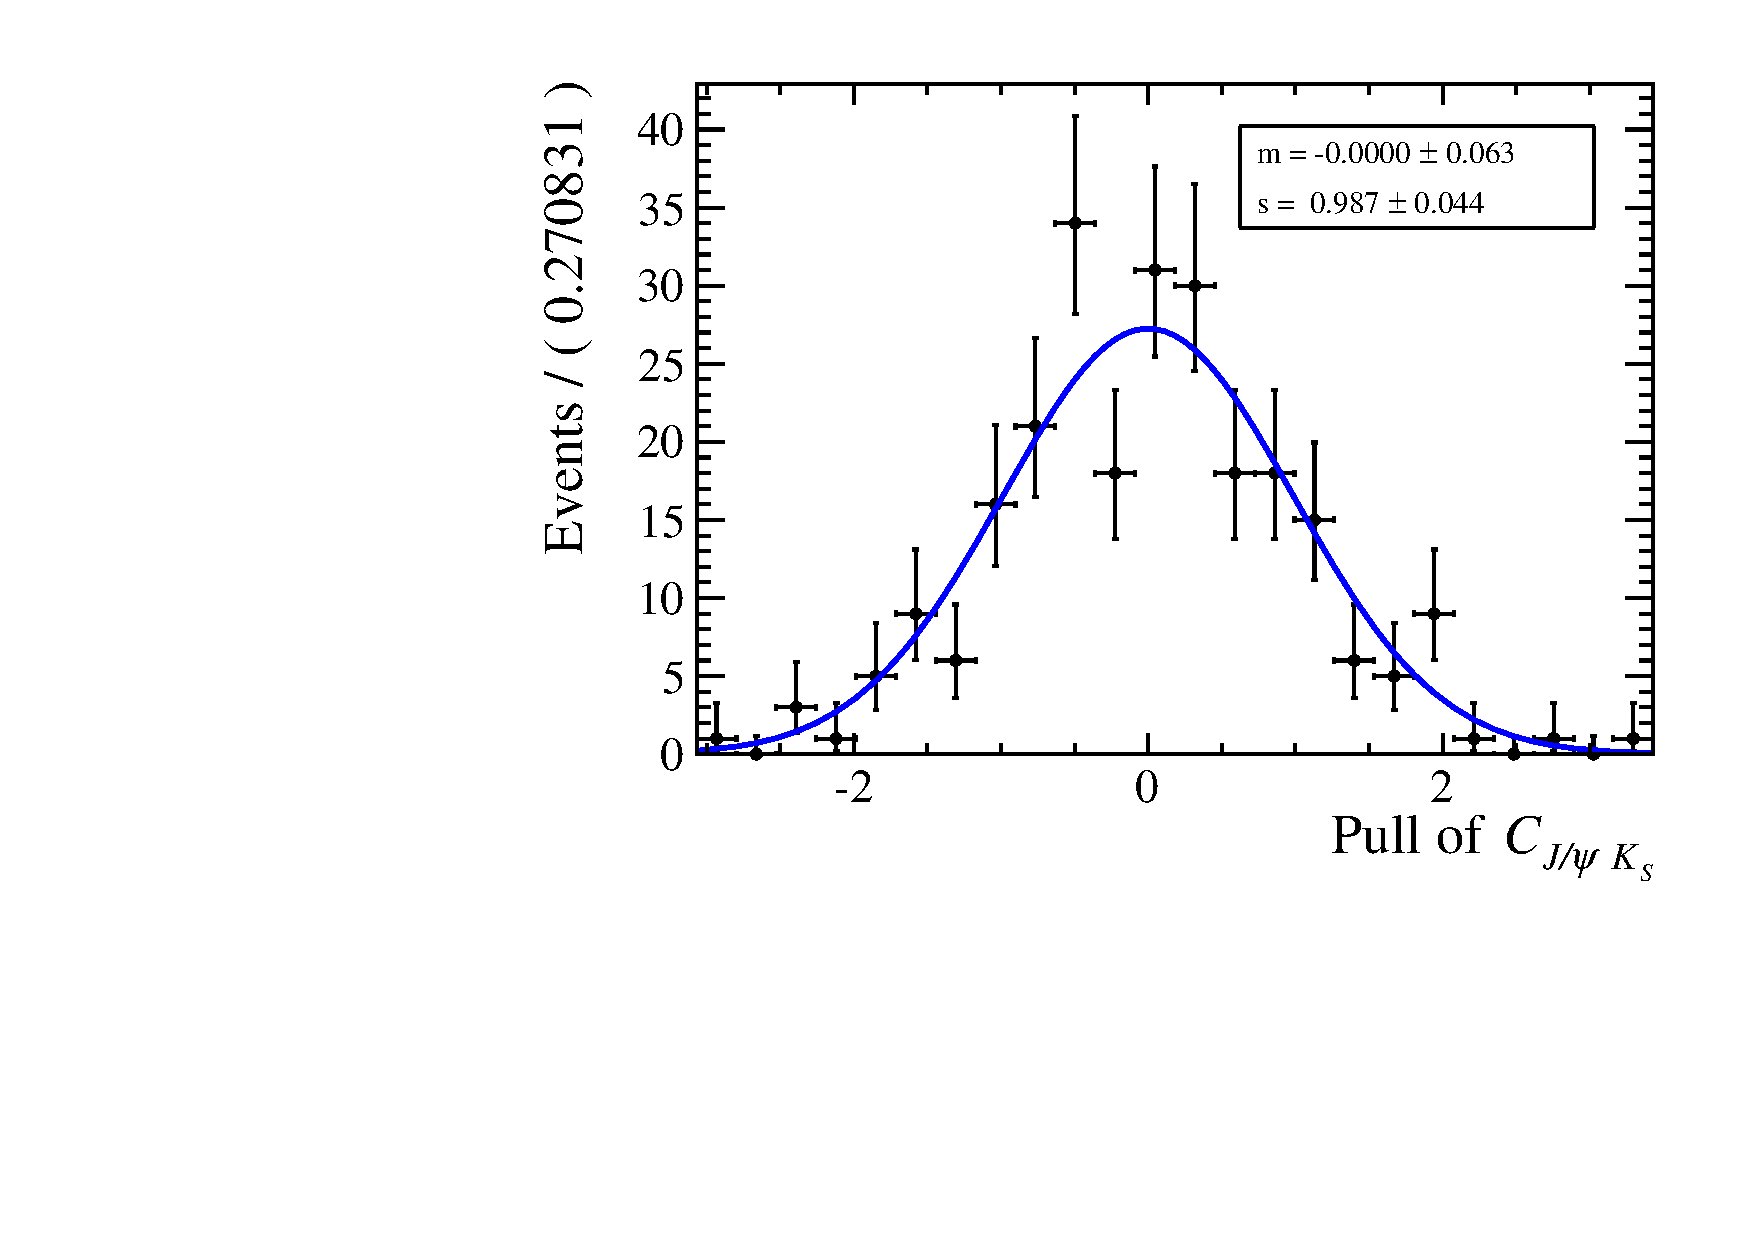
\includegraphics[width=0.49\textwidth]{private/content/measurement-of-sin2beta/figs/systematics_acc_lower_c_pull.pdf}\hfill
  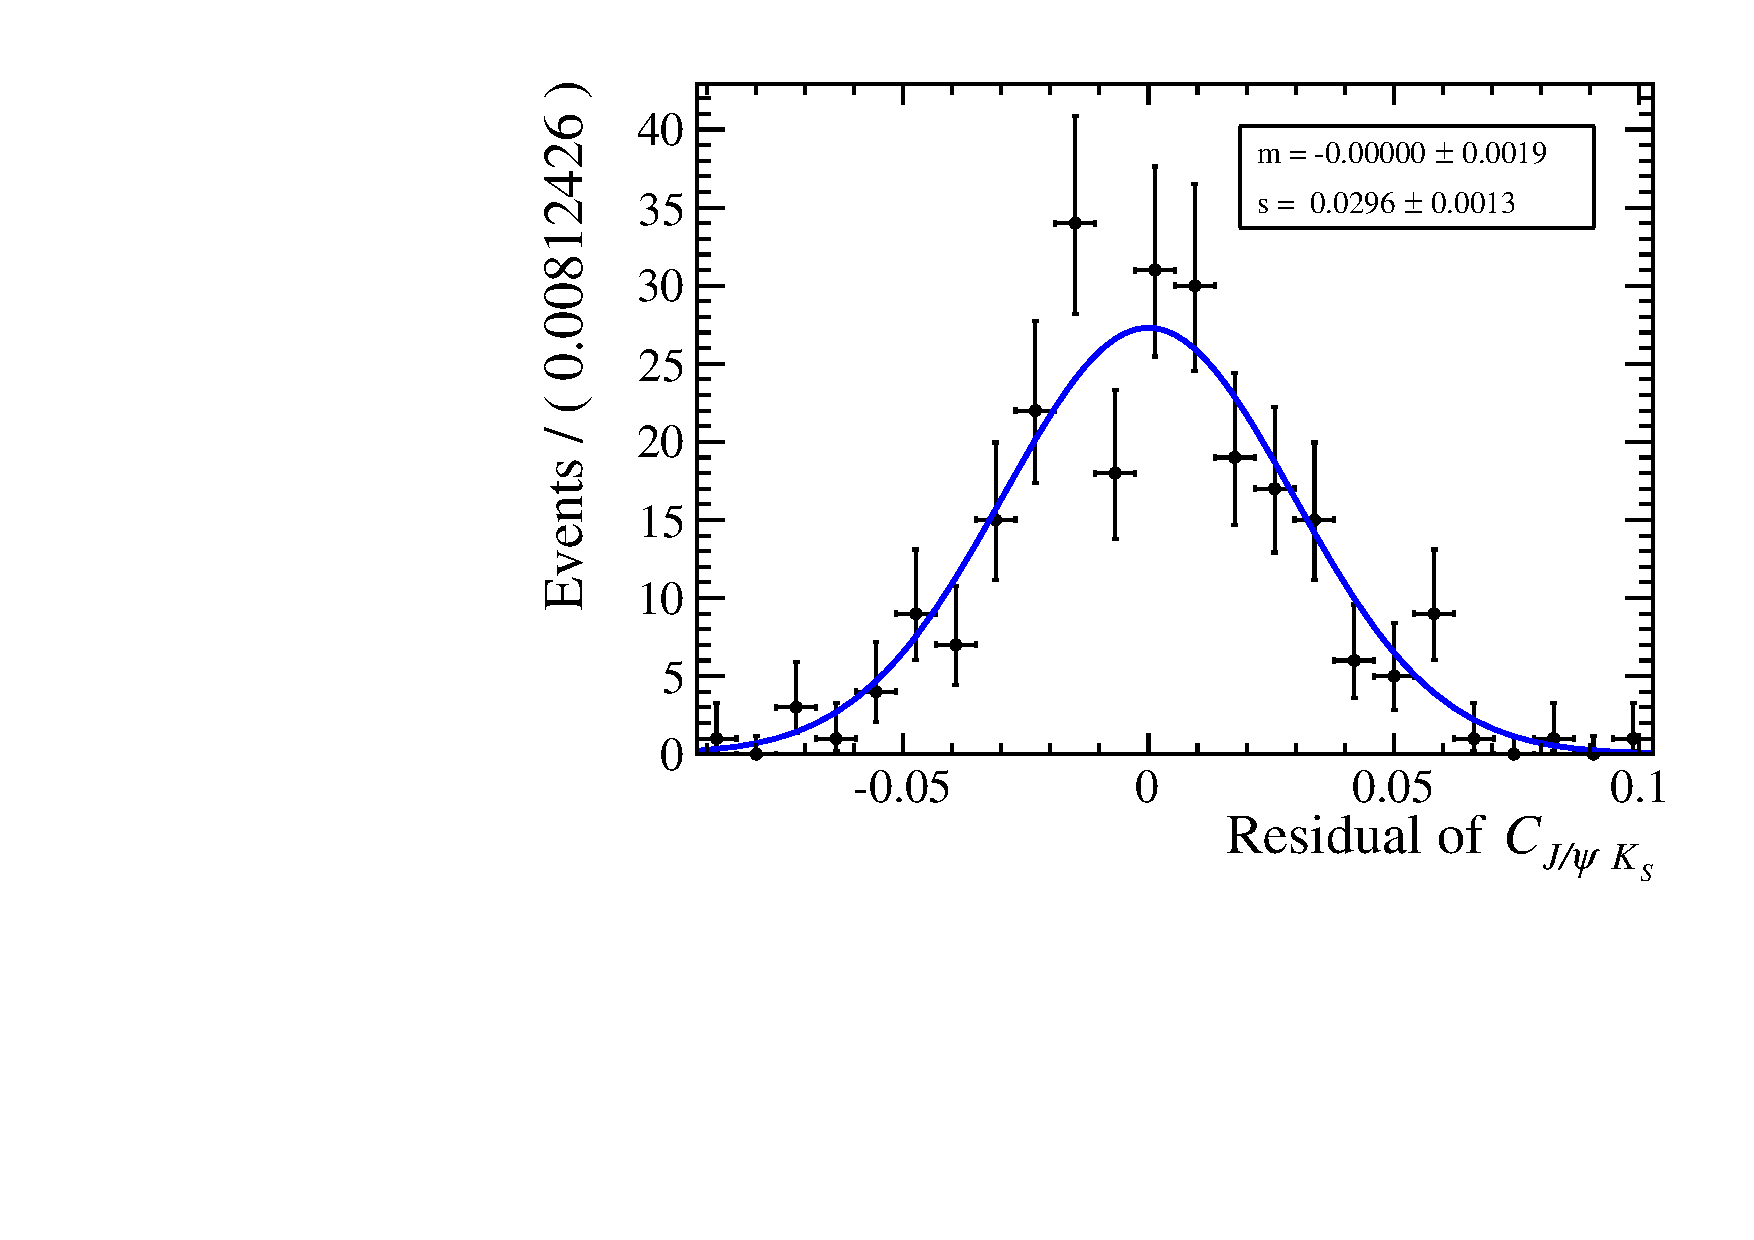
\includegraphics[width=0.49\textwidth]{private/content/measurement-of-sin2beta/figs/systematics_acc_lower_c_res.pdf}
\caption{Shown are (left) pull and (right) residual distributions of the
parameters (top) \SJpsiKS and (bottom) \CJpsiKS from a \ToyMC study of the
influence of the low decay time acceptance model on the \CP parameters.}
\label{fig:app:measurement_of_sin2beta:systematics:systematics:acceptance:lower}
\end{figure}

% ..............................................................................
\subsection{Upper decay time acceptance}
\label{sec:app:measurement_of_sin2beta:systematics:systematics:acceptance:upper}

\begin{figure}[h]
  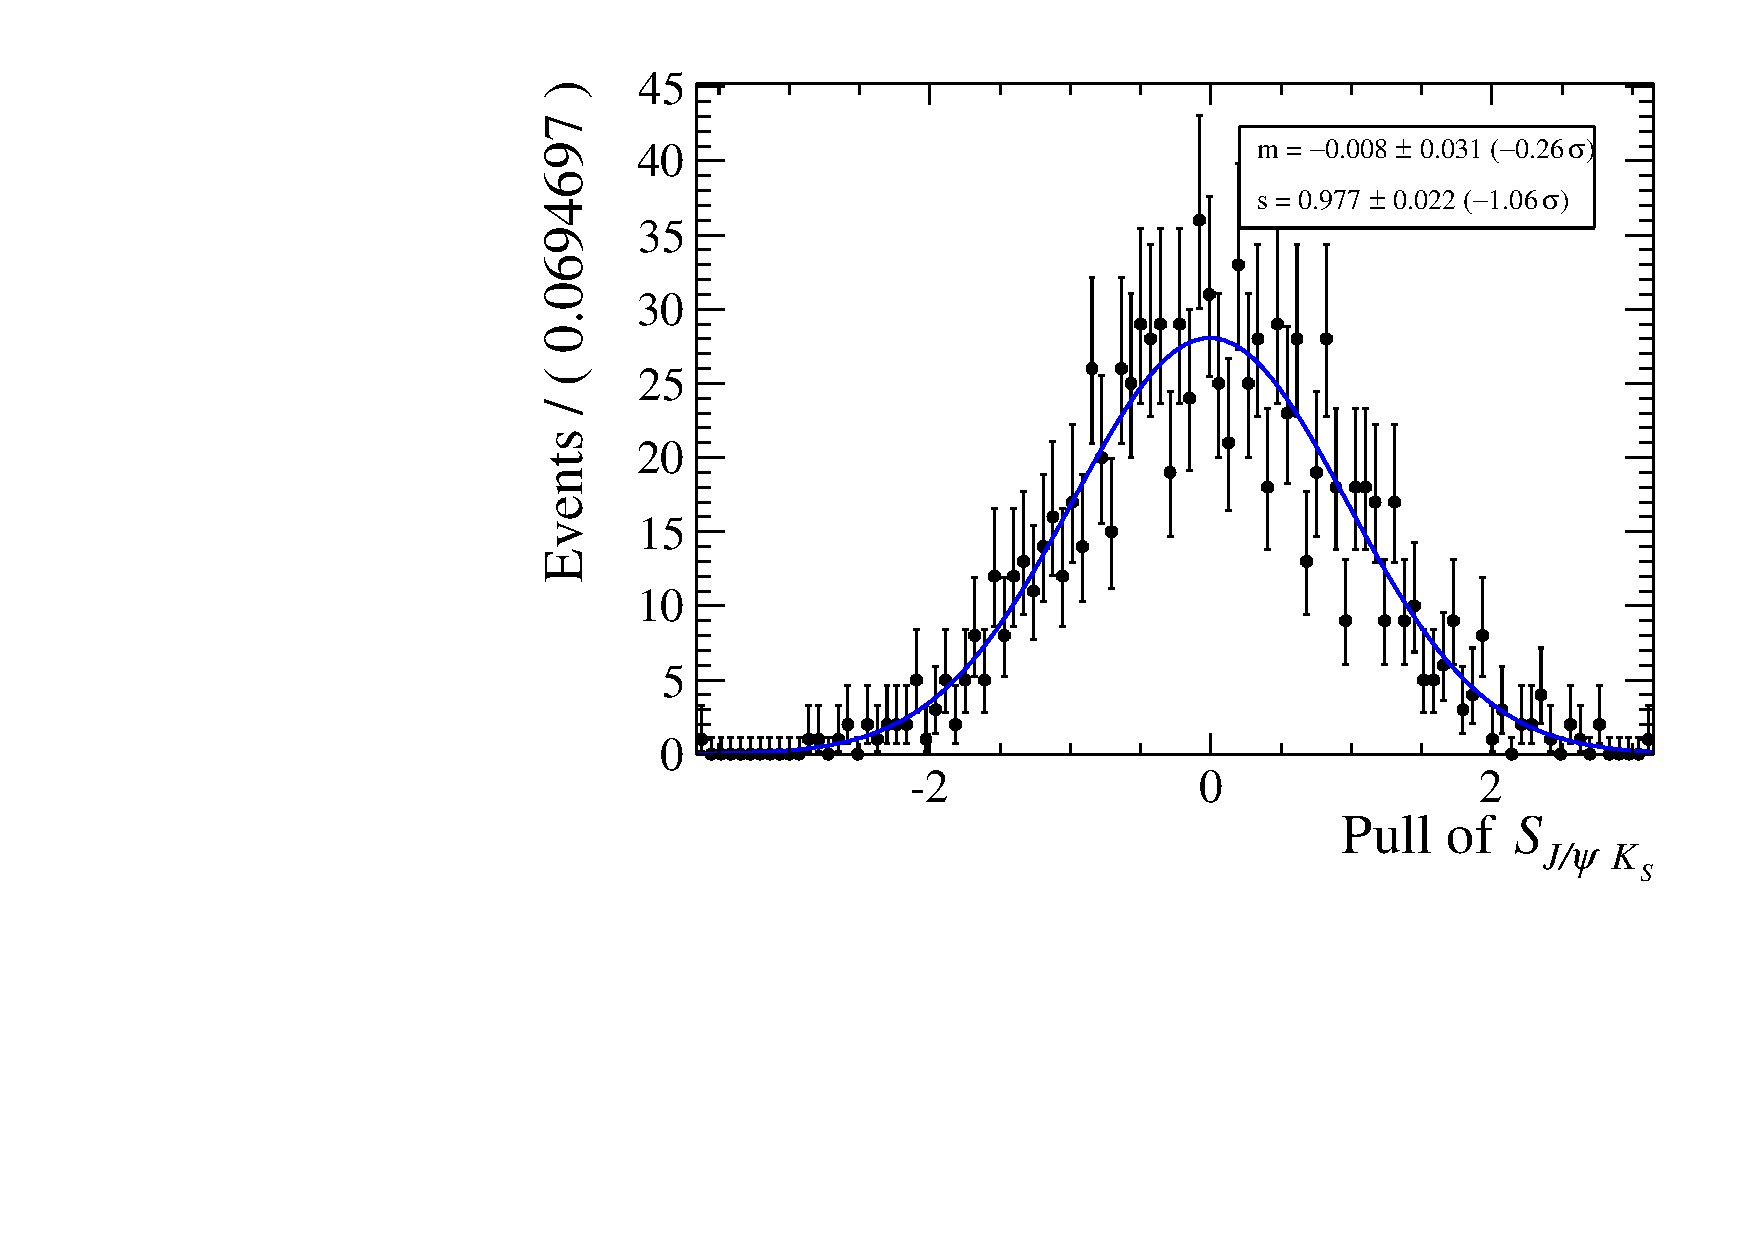
\includegraphics[width=0.49\textwidth]{private/content/measurement-of-sin2beta/figs/systematics_acc_upper_s_pull.pdf}\hfill
  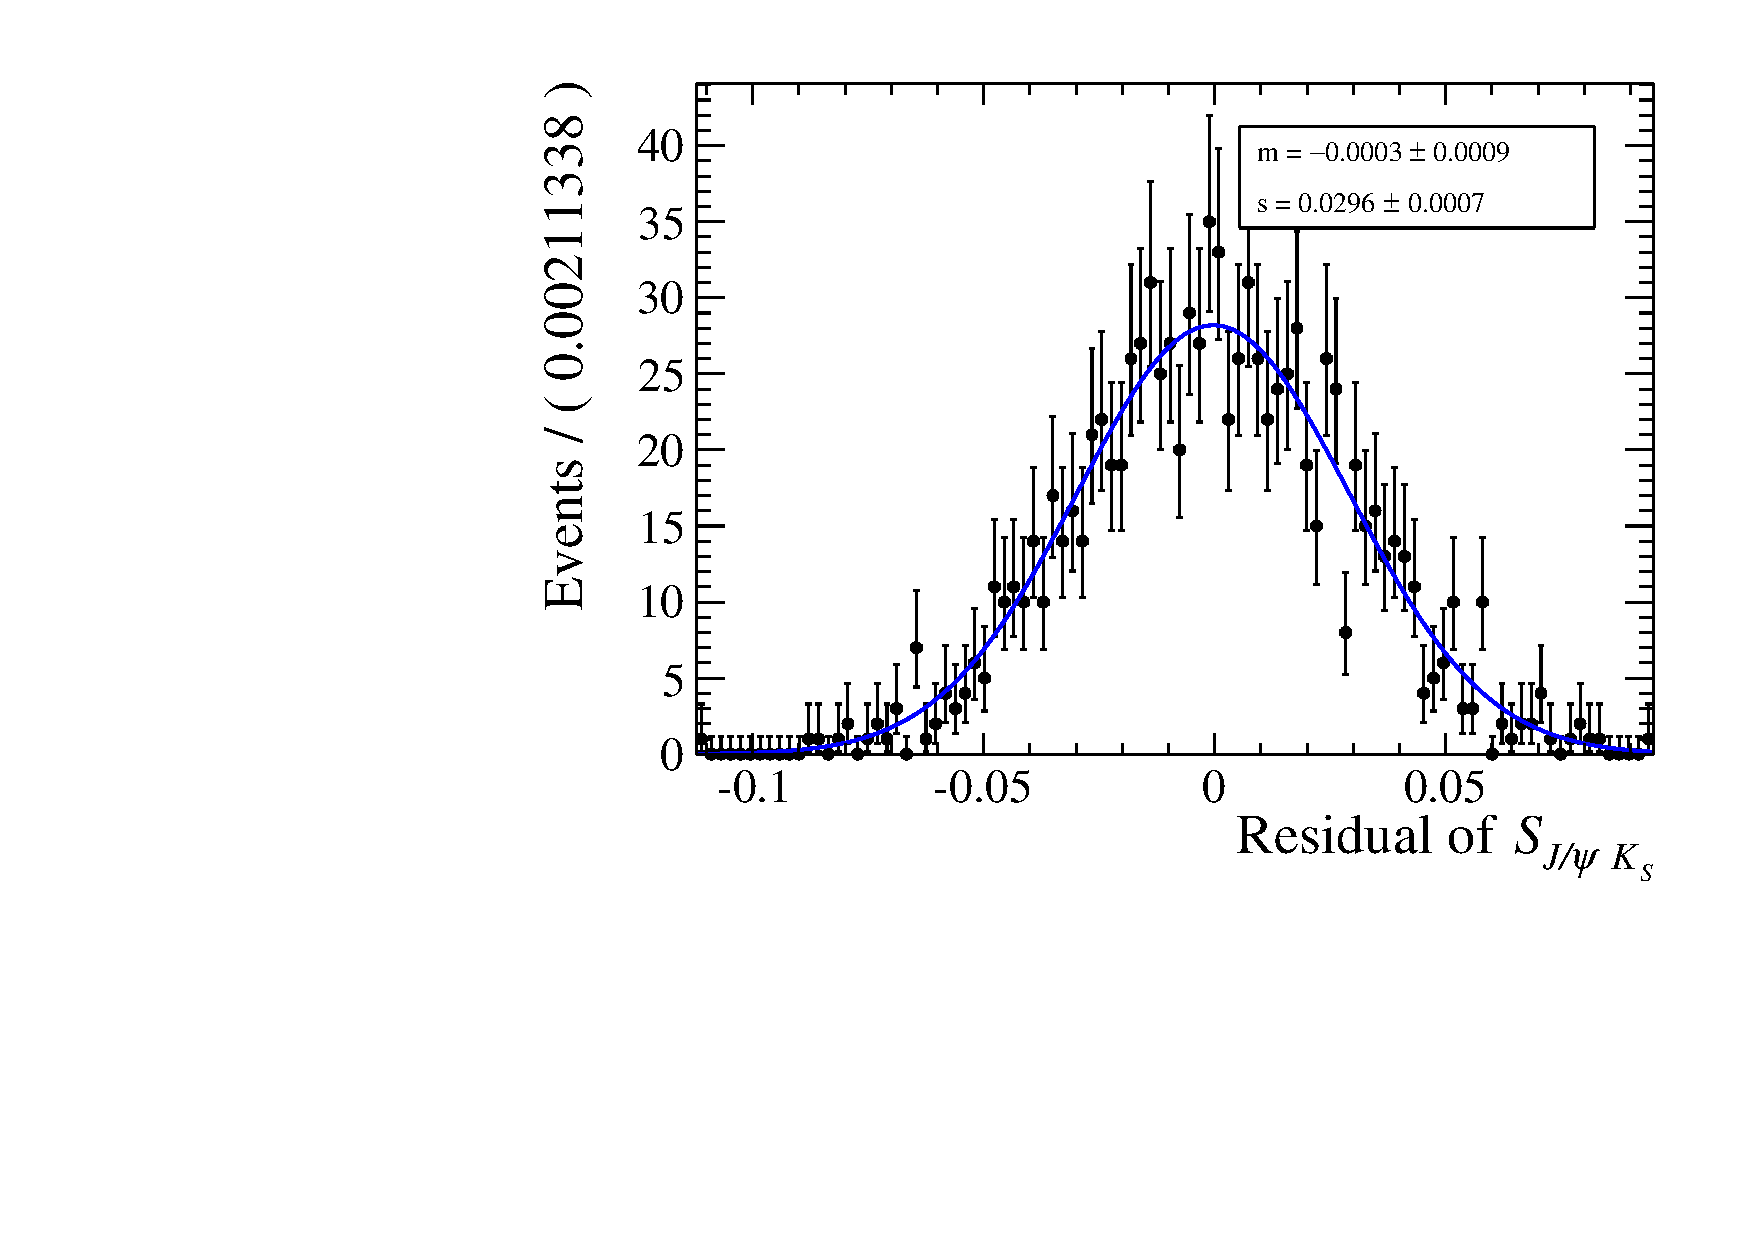
\includegraphics[width=0.49\textwidth]{private/content/measurement-of-sin2beta/figs/systematics_acc_upper_s_res.pdf}
  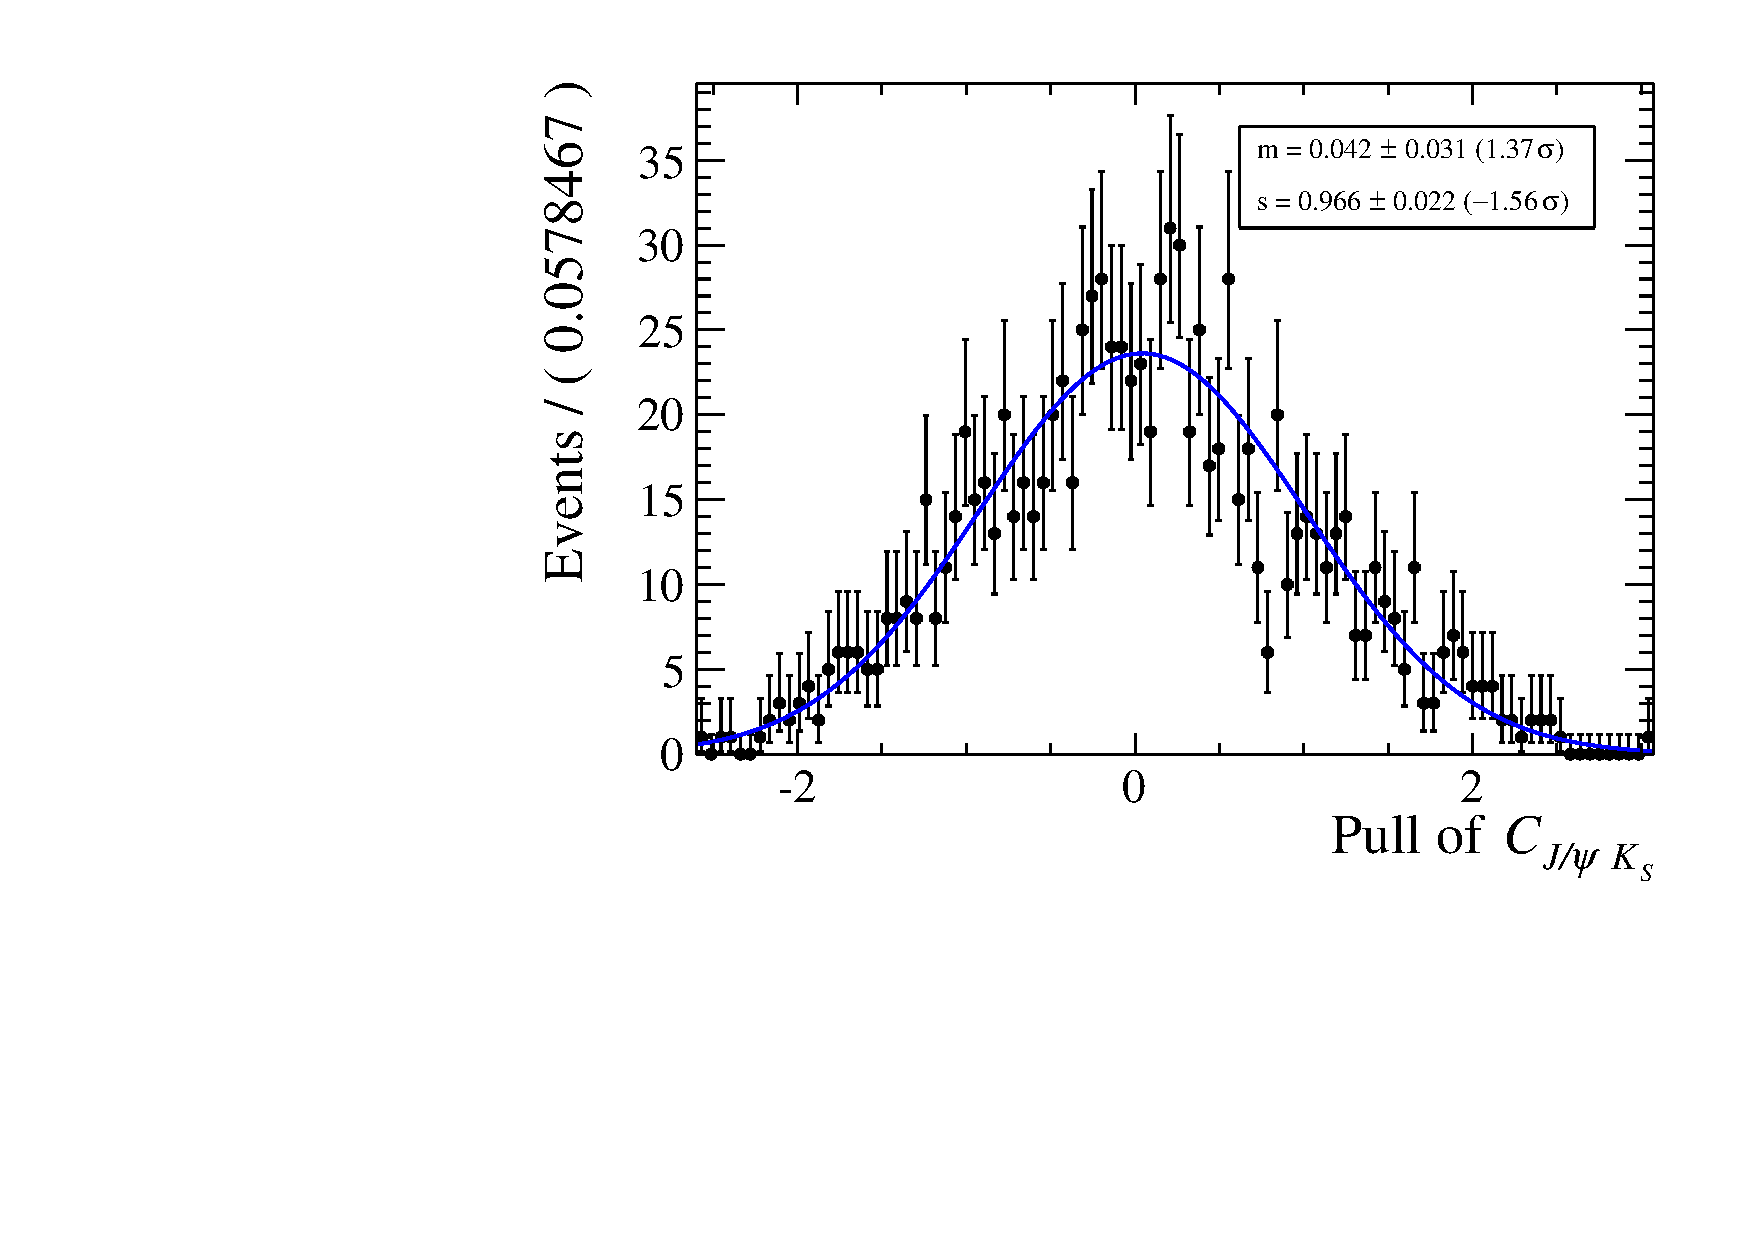
\includegraphics[width=0.49\textwidth]{private/content/measurement-of-sin2beta/figs/systematics_acc_upper_c_pull.pdf}\hfill
  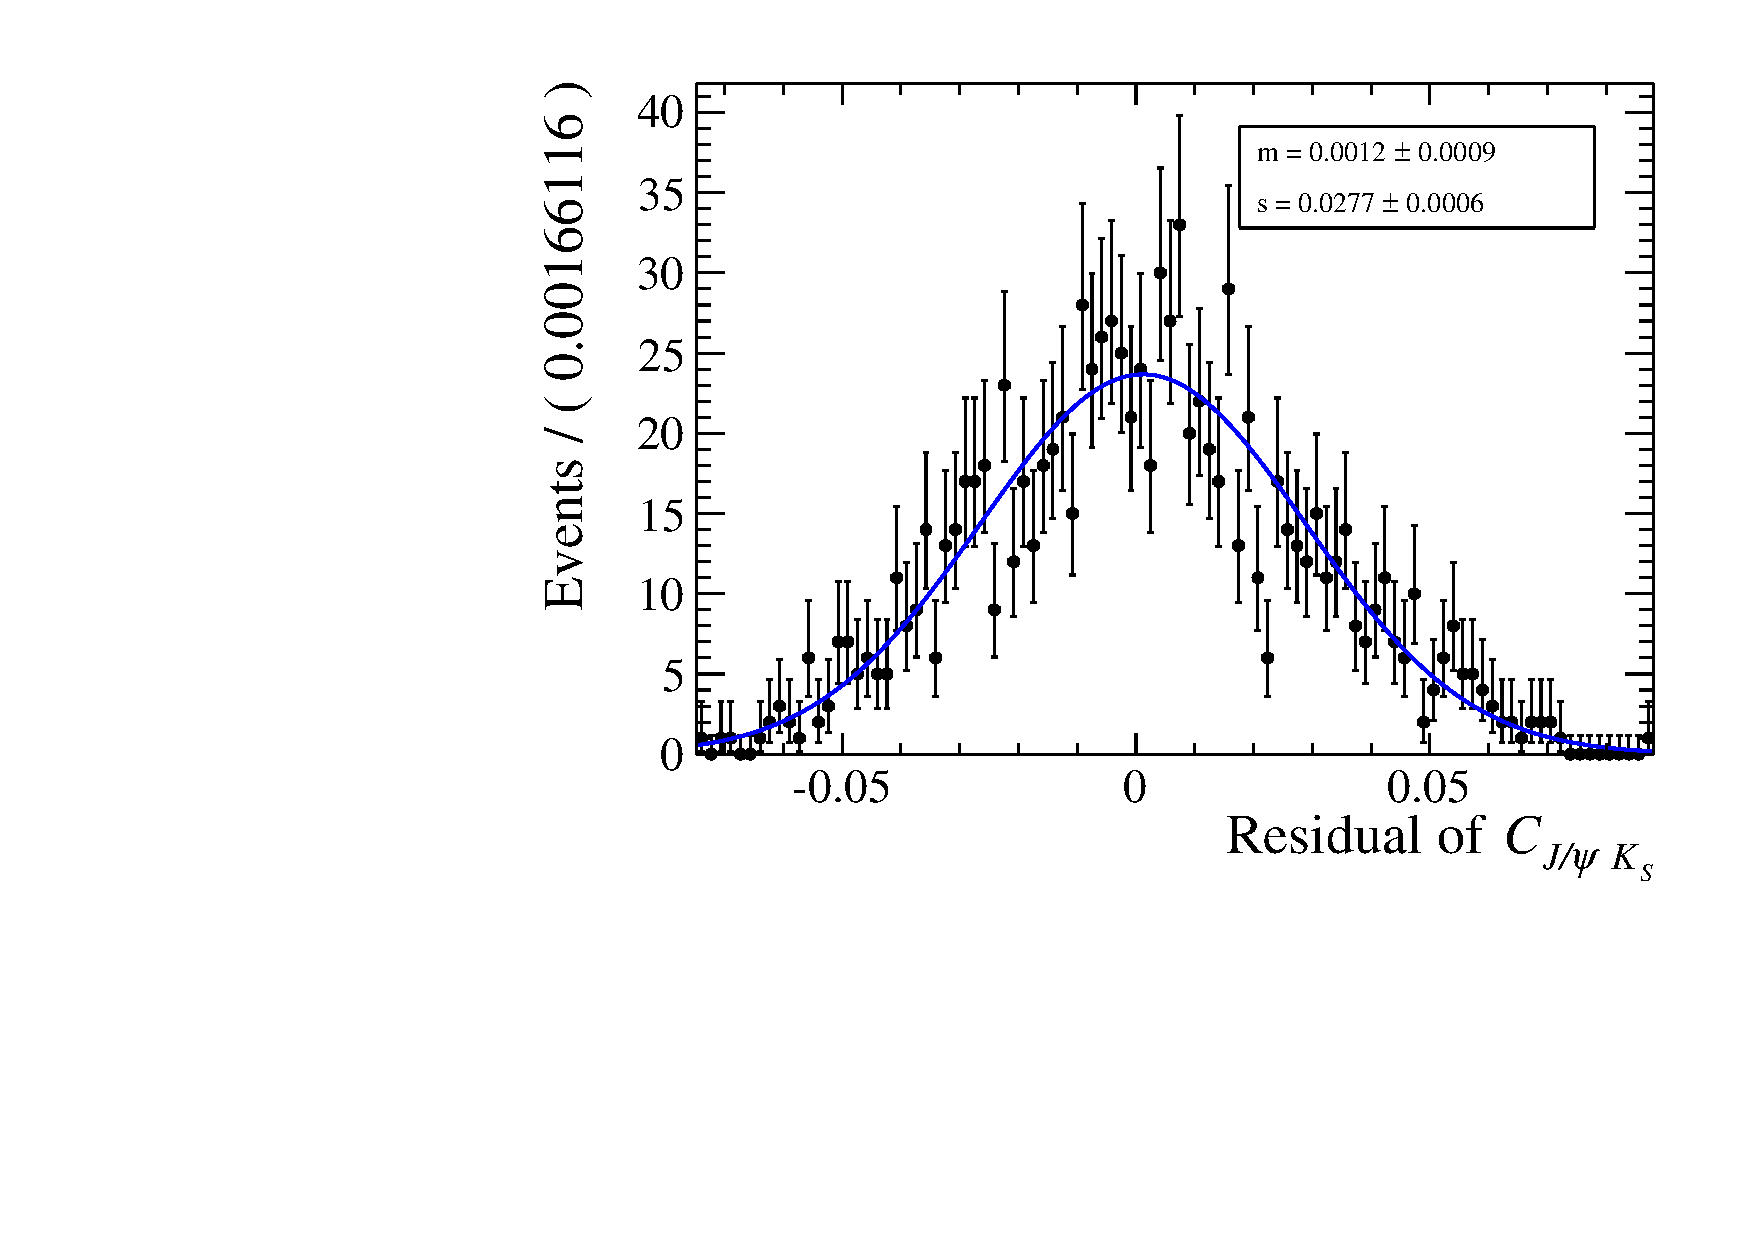
\includegraphics[width=0.49\textwidth]{private/content/measurement-of-sin2beta/figs/systematics_acc_upper_c_res.pdf}
\caption{Shown are (left) pull and (right) residual distributions of the
parameters (top) \SJpsiKS and (bottom) \CJpsiKS from a \ToyMC study of the
influence of the upper decay time acceptance correction function on the \CP
parameters.}
\label{fig:app:measurement_of_sin2beta:systematics:systematics:acceptance:upper}
\end{figure}

% ------------------------------------------------------------------------------
\subsection[Production asymmetry, $z$-scale, DMd, and DGd]{Production asymmetry, $z$-scale, \DMd, and \DGd}
\label{sec:app:measurement_of_sin2beta:systematics:systematics:further_studies}
